\documentclass[12pt,a4paper]{article}
\usepackage{cmap} % Makes the PDF copiable. See http://tex.stackexchange.com/a/64198/25761
\usepackage[T1]{fontenc}
\usepackage[brazil]{babel}
\usepackage[utf8]{inputenc}
\usepackage{amsmath}
\usepackage{amsfonts}
\usepackage{amssymb}
\usepackage{amsthm}
\usepackage[usenames,svgnames,dvipsnames]{xcolor}
\usepackage{hyperref}
\usepackage{multicol}
\usepackage{graphicx}
\usepackage[margin=2cm]{geometry}
\usepackage{systeme}
\usepackage{cancel}
\usepackage{icomma}

\hypersetup{
    colorlinks = true,
    allcolors = {blue}
}

% TODO: Consider using exsheets
% http://linorg.usp.br/CTAN/macros/latex/contrib/exsheets/exsheets_en.pdf
%
% http://ctan.org/tex-archive/macros/latex/contrib/exercise/
% Options: answerdelayed,lastexercise,noanswer
\usepackage[answerdelayed,lastexercise]{exercise}

\addto\captionsbrazil{%
\def\listexercisename{Lista de exerc\'icios}%
\def\ExerciseName{Exerc\'icio}%
\def\AnswerName{Solu\c{c}\~ao do exerc\'icio}%
\def\ExerciseListName{Ex.}%
\def\AnswerListName{Solu\c{c}\~ao}%
\def\ExePartName{Parte}%
\def\ArticleOf{de\ }%
}

\renewcommand{\ExerciseHeaderTitle}{(\ExerciseTitle)\ }
\renewcommand{\ExerciseListHeader}{%\ExerciseHeaderDifficulty%
\textbf{%\ExerciseListName\
\ExerciseHeaderNB.\ %
%\ --- \
\ExerciseHeaderTitle}%
%\ExerciseHeaderOrigin
\ignorespaces}
\renewcommand{\AnswerListHeader}{\textbf{\ExerciseHeaderNB.\ (\AnswerListName)\ }}

\newcommand*\diff{\mathop{}\!\mathrm{d}}
\newcommand*\sen{\operatorname{sen}}
\newcommand*\dom[1]{\operatorname{Dom}\left(#1\right)}

\newcommand*\R{\mathbb{R}}

\renewcommand{\theenumi}{\alph{enumi}}
\renewcommand\labelenumi{(\theenumi) }

\newcommand*\tipo{Prova III}
\newcommand*\turma{NEXM241-A}
\newcommand*\disciplina{CDI2001}
\newcommand*\eu{Helder G. G. de Lima}
\newcommand*\data{08/06/2024}

\author{\eu}
\title{\tipo - \disciplina}
\date{\data}

\begin{document}
\thispagestyle{empty}
\newgeometry{margin=2cm,bottom=0.5cm}
\begin{center}

\includegraphics[width=9.0cm]{marca} \\
\textbf{\tipo\ (\disciplina / \turma)} \\
Prof. \eu\footnote{
Este é um material de acesso livre distribuído sob os termos da licença \href{https://creativecommons.org/licenses/by-sa/4.0/deed.pt_BR}{Creative Commons BY-SA 4.0}}
\end{center}

\noindent Nome do(a) aluno(a): \underline{\hspace{9,7cm}} Data: \underline{\data}

%\section*{Instruções}
\begin{center}\fbox{
\begin{minipage}{14cm}

{\footnotesize
\begin{itemize}
\renewcommand{\theenumi}{\Roman{enumi}}
\item Identifique-se em todas as folhas.
\item Não é permitido o uso de calculadora.
\item Mantenha o celular e os demais equipamentos eletrônicos desligados durante a prova.
\item Justifique cada resposta com cálculos ou argumentos baseados na teoria estudada.
\item Resolva $5$ das $6$ questões (deixe claro que questão não deverá ser corrigida).
\end{itemize}
}

\end{minipage}
}
\end{center}

%\section*{Questões}
\begin{ExerciseList}
\Exercise[title={2,0}] Estime $\sqrt{(6,02)^2 + (7,99)^2}$ usando o conceito de diferencial ou de aproximação linear.
\Answer Considerando $z = f(x, y) = \sqrt{x^2 + y^2}$, o objetivo é obter o valor aproximado de $f(6,02, 7,99)$. Como $(6,02, 7,99)$ está próximo do ponto $(6, 8)$, pode-se obter a aproximação linear de $f$ em $(6, 8)$, e usá-la para estimar o valor procurado, já que para pontos $(x, y)$ em uma vizinhança de $(6, 8)$, tem-se:
\[
  f(x, y) \approx f(6, 8) + \frac{\partial f}{\partial x}(6, 8)(x - 6) + \frac{\partial f}{\partial y}(6, 8)(y - 8).
\]
Mas $f(6, 8) = \sqrt{6^2 + 8^2} = \sqrt{36 + 64} = \sqrt{100} = 10$ e para todo $(x, y) \neq (0, 0)$, tem-se
\[
  \frac{\partial f}{\partial x}(x, y)
  = \frac{2x}{2\sqrt{x^2 + y^2}}
  = \frac{x}{\sqrt{x^2 + y^2}}
  \quad\text{ e }\quad
  \frac{\partial f}{\partial y}(x, y)
  = \frac{2y}{2\sqrt{x^2 + y^2}}
  = \frac{y}{\sqrt{x^2 + y^2}}.
\]
Em particular, $\frac{\partial f}{\partial x}(6, 8) = \frac{6}{\sqrt{6^2 + 8^2}} = \frac{6}{10}$ e $\frac{\partial f}{\partial x}(x, y) = \frac{8}{\sqrt{6^2 + 8^2}} = \frac{8}{10}$. Portanto,
\begin{align*}
  \sqrt{(6,02)^2 + (7,99)^2}
  & = f(6,02, 7,99)
    = 10 + \frac{6}{10}(6,02 - 6) + \frac{8}{10}(7,99 - 8) \\
  & = 10 + \frac{6}{10} \cdot 0,02 + \frac{8}{10}\cdot (-0,01)
    = 10 + \frac{0,12 - 0,08}{10}
    = 10 + \frac{0,04}{10} \\
  & = 10 + 0,004
    = 10,004.
\end{align*}
\textit{Observação}: Apenas para fins de comparação, o valor exato, arredondado com seis dígitos corretos após a vírgula é $\sqrt{1000805}/100 \approx \textbf{10,004}024$.


\Exercise[title={2,0}] Determine, caso existam, os pontos críticos da função $f(x,y) = 6\ln(x)+\frac{12}{y} + xy$, e classifique-os, se possível, como pontos de máximo, mínimo ou de sela.
\Answer Observe que $\dom{f} = \{(x,y) \in \R^2 \mid x > 0 \text{ e } y \neq 0 \}$. Além disso, as derivadas parciais de primeira ordem de $f$ são:
\[
  \frac{\partial f}{\partial x}(x, y) = \frac{6}{x} + y
  \quad\text{ e }\quad
  \frac{\partial f}{\partial y}(x, y) = -\frac{12}{y^2} + x.
\]
Para que $(x, y)$ seja um ponto crítico de $f$, as derivadas parciais devem ser nulas ou inexistentes. Mas as derivadas parciais estão definidas em todo $(x, y) \in \dom{f}$, e
\[
  \begin{cases}
    \frac{6}{x} + y = 0 \\
    -\frac{12}{y^2} + x = 0
    \end{cases}
  \Leftrightarrow
  \begin{cases}
    y = -\frac{6}{x} \\
    x = \frac{12}{y^2}.
    \end{cases}
\]
Substituindo o valor de $y$ da primeira equação na segunda equação, resulta que
\[
  x
  = \frac{12}{y^2}
  = \frac{12}{\left(-\frac{6}{x}\right)^2}
  = \frac{12}{\frac{36}{x^2}}
  = 12 \cdot \frac{x^2}{36}
  = \frac{x^2}{3}
  \quad\Rightarrow\quad
  \frac{x^2}{3} - x = 0
  \Rightarrow
  x\left(\frac{x}{3} - 1\right) = 0.
\]
Como nenhum $(x, y)$ com $x=0$ está no domínio de $f$, conclui-se que $\frac{x}{3} - 1 = 0$, isto é, $x = 3$. Consequentemente, $y = -\frac{6}{3} = -2$ e o único ponto crítico é $(3, -2)$ (como prova real, observe que esse ponto realmente satisfaz $\frac{\partial f}{\partial x}(3, -2) = \frac{6}{3} + (-2) = 0$ e $\frac{\partial f}{\partial y}(3, -2) = -\frac{12}{(-2)^2} + 3 = 0$). Para classificá-lo, considere
\[
H(x, y) =
\begin{vmatrix}
  \frac{\partial^2 f}{\partial x^2}(x, y) & \frac{\partial^2 f}{\partial y \partial x}(x, y) \\
  \frac{\partial^2 f}{\partial x\partial y}(x, y) & \frac{\partial^2 f}{\partial y^2}(x, y)
\end{vmatrix}
=
\begin{vmatrix}
  \frac{-6}{x^2} & 1 \\
  1 & \frac{24}{y^3}
\end{vmatrix}
= -\frac{144}{x^2y^3} - 1.
\]
Como $H(3, -2) = \begin{vmatrix}
  \frac{-6}{3^2} & 1 \\
  1 & \frac{24}{(-2)^3}
\end{vmatrix} = -\frac{144}{9 \cdot (-8)} - 1 = 1 > 0$, e $\frac{\partial^2 f}{\partial x^2}(x, y) = \frac{-6}{3^2} = -\frac{2}{3} < 0$, conclui-se que o ponto crítico $(3, -2)$ é um ponto de máximo local de $f$, como pode ser confirmado na figura a seguir:


\begin{center}
  \includegraphics[width=5.0cm]{img/prova-3-nex-ponto-crítico.png}
\end{center}

\Exercise[title={2,0}] Utilize a teoria e os conceitos de cálculo diferencial para determinar o ponto do eixo $x$ que está mais próximo da reta $r: (x, y, z) = (1, 2, 3) + \beta (-1, 1, 0)$.

\textit{Dica: É conveniente considerar o quadrado da distância entre um ponto do eixo $x$ e um de $r$.}

\Answer A distância entre um ponto $A = (\alpha, 0, 0)$ do eixo $x$ e um ponto $B = (1 - \beta, 2 + \beta, 3)$ da reta $r$ depende dos parâmetros $\alpha$ e $\beta$ que determinam esses pontos, e é dada por:
\[
d
= \sqrt{(1 - \beta - \alpha)^2 + (2 + \beta)^2 + (3 - 0)^2}.
\]
Para obter o ponto do eixo $x$ que está mais próximo próximo de $r$, basta determinar os valores de $\alpha$ e $\beta$ que minimizam $d$ ou, equivalentemente, que minimizam $d^2$. Considere a função
\[
  f(\alpha, \beta) = (1 - \beta - \alpha)^2 + (2 + \beta)^2 + 9.
\]

Então, como $f$ é derivável, seus pontos críticos anulam suas derivadas parciais:
\[
  0 = \frac{\partial f}{\partial \alpha}(\alpha, \beta)
  = 2(1 - \beta - \alpha)(-1)
  = 2\alpha + 2\beta - 2
  \Leftrightarrow
  \alpha + \beta - 1 = 0
\]
e
\[
  0 = \frac{\partial f}{\partial \beta}(\alpha, \beta)
  = 2(1 - \beta - \alpha)(-1) + 2(2 + \beta)
  = 2\alpha + 4\beta + 2
  \Leftrightarrow
  \alpha + 2\beta + 1 = 0
\]
Assim, $\alpha$ e $\beta$ devem ser soluções do sistema linear
\[
\begin{cases}
  \alpha + \beta = 1\\
  \alpha + 2\beta = -1\\
\end{cases}
\Rightarrow
\beta = -2
\Rightarrow
\alpha = 3,
\]
Como a solução é única, $f$ tem um único ponto crítico, que pode ser visto no seguinte gráfico:

\begin{center}
  \includegraphics[width=8.0cm]{img/prova-3-nex-distância.png}
\end{center}

No contexto original, isso quer dizer que o ponto $A = (\alpha, 0, 0) = (3, 0, 0)$ é o único candidato a ser o ponto mais próximo da reta $r$, conforme é mostrado na figura a seguir:

\begin{center}
  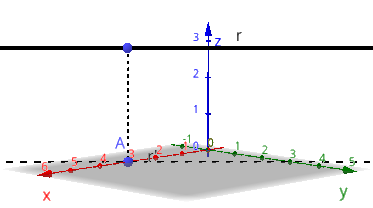
\includegraphics[width=7.0cm]{img/prova-3-nex-reta.png}
\end{center}

Resta verificar que o ponto crítico $C = (3, -2)$ realmente é um ponto de mínimo de $f(\alpha, \beta)$:\[
H(x, y) =
\begin{vmatrix}
  \frac{\partial^2 f}{\partial x^2}(x, y) & \frac{\partial^2 f}{\partial y \partial x}(x, y) \\
  \frac{\partial^2 f}{\partial x\partial y}(x, y) & \frac{\partial^2 f}{\partial y^2}(x, y)
\end{vmatrix}
=
\begin{vmatrix}
  2 & 2 \\
  2 & 4
\end{vmatrix}
= 8 - 4 = 4 > 0.
\]
Como $H(3, -2) = 4 > 0$, e $\frac{\partial^2 f}{\partial x^2}(x, y) = 2 > 0$, então $(3, -2)$ é um ponto de mínimo de $f$.


\Exercise[title={2,0}] Calcule a integral iterada $\int_0^{\sqrt{\pi}}\int_{x}^{\sqrt{\pi}} 2\cos\left(y^2\right) \diff{y}\diff{x}$.
\Answer Seja $D	= \{(x, y) \in \mathbb{R} \mid 0 \leq x \leq \sqrt{\pi} \text{ e } x \leq y \leq \sqrt{\pi} \}$, conforme a figura a seguir:

\begin{center}
  \includegraphics[width=5.0cm]{img/prova-3-nex-integral-iterada-domínio.pdf}
\end{center}

Para essa representação, basta considerar que $1 \leq \sqrt{\pi} \leq 2$ (pois $1 \leq \pi \leq 4$). Assim:
\[
\int_0^{\sqrt{\pi}}\int_{x}^{\sqrt{\pi}} 2\cos\left(y^2\right) \diff{y}\diff{x}
 = \iint_{D} \cos\left(y^2\right) \diff{A}.
\]

Reescrevendo $D = \{(x, y) \in \mathbb{R} \mid 0 \leq y \leq \sqrt{\pi} \text{ e } 0 \leq x \leq y \}$, obtém-se:
\begin{align*}
\iint_{D} 2\cos\left(y^2\right() \diff{A}
& = \int_0^{\sqrt{\pi}}\int_0^{y} 2\cos\left(y^2\right) \diff{x}\diff{y}
  = \int_0^{\sqrt{\pi}} \left.\left(2x\cos\left(y^2\right)\right)\right|_{x=0}^{x=y}\diff{y} \\
& = \int_0^{\sqrt{\pi}} 2y\cos\left(y^2\right) - 0\diff{y}
  = \left.\sen\left(y^2\right)\right|_{y=0}^{y=\sqrt{\pi}} \\
& = \sen\left(\left(\sqrt{\pi}\right)^2\right) - \sen\left(0^2\right)
  = 0 - 0
  = 0.
\end{align*}

O gráfico da função $f(x,y) = \cos(y^2)$, restrita ao conjunto $D$, é mostrado a seguir:
\begin{center}
  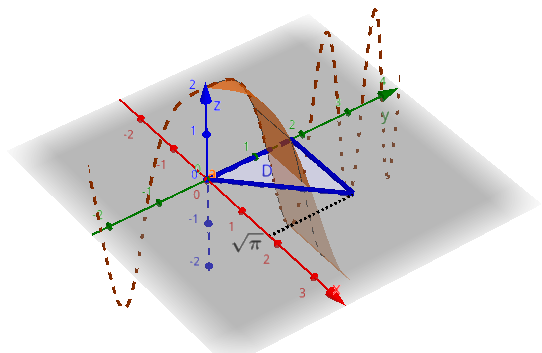
\includegraphics[width=7.0cm]{img/prova-3-nex-integral-iterada.png}
\end{center}

Note que há partes do gráfico tanto acima quanto abaixo do plano $z = 0$, o que torna plausível que a integral seja nula, já que o volume acima do plano $z = 0$ cancela o que está abaixo.


\Exercise[title={2,0}] Represente graficamente o sólido $S$ definido por $x^2 + y^2 + z^2 \leq 1$ e $z \geq \sqrt{x^2 + y^2}$ e utilize coordenadas esféricas para calcular a integral tripla $\iiint_{S} z \diff{V}$.
\Answer A condição $x^2 + y^2 + z^2 \leq 1$ corresponde ao interior de uma esfera de raio um centrada na origem, e a desigualdade $z \geq \sqrt{x^2 + y^2}$ é satisfeita pelos pontos que estão acima de um cone com vértice na origem e cujo eixo de simetria é o eixo $z$. Assim, o sólido $S$ tem a seguinte representação geométrica:

\begin{center}
  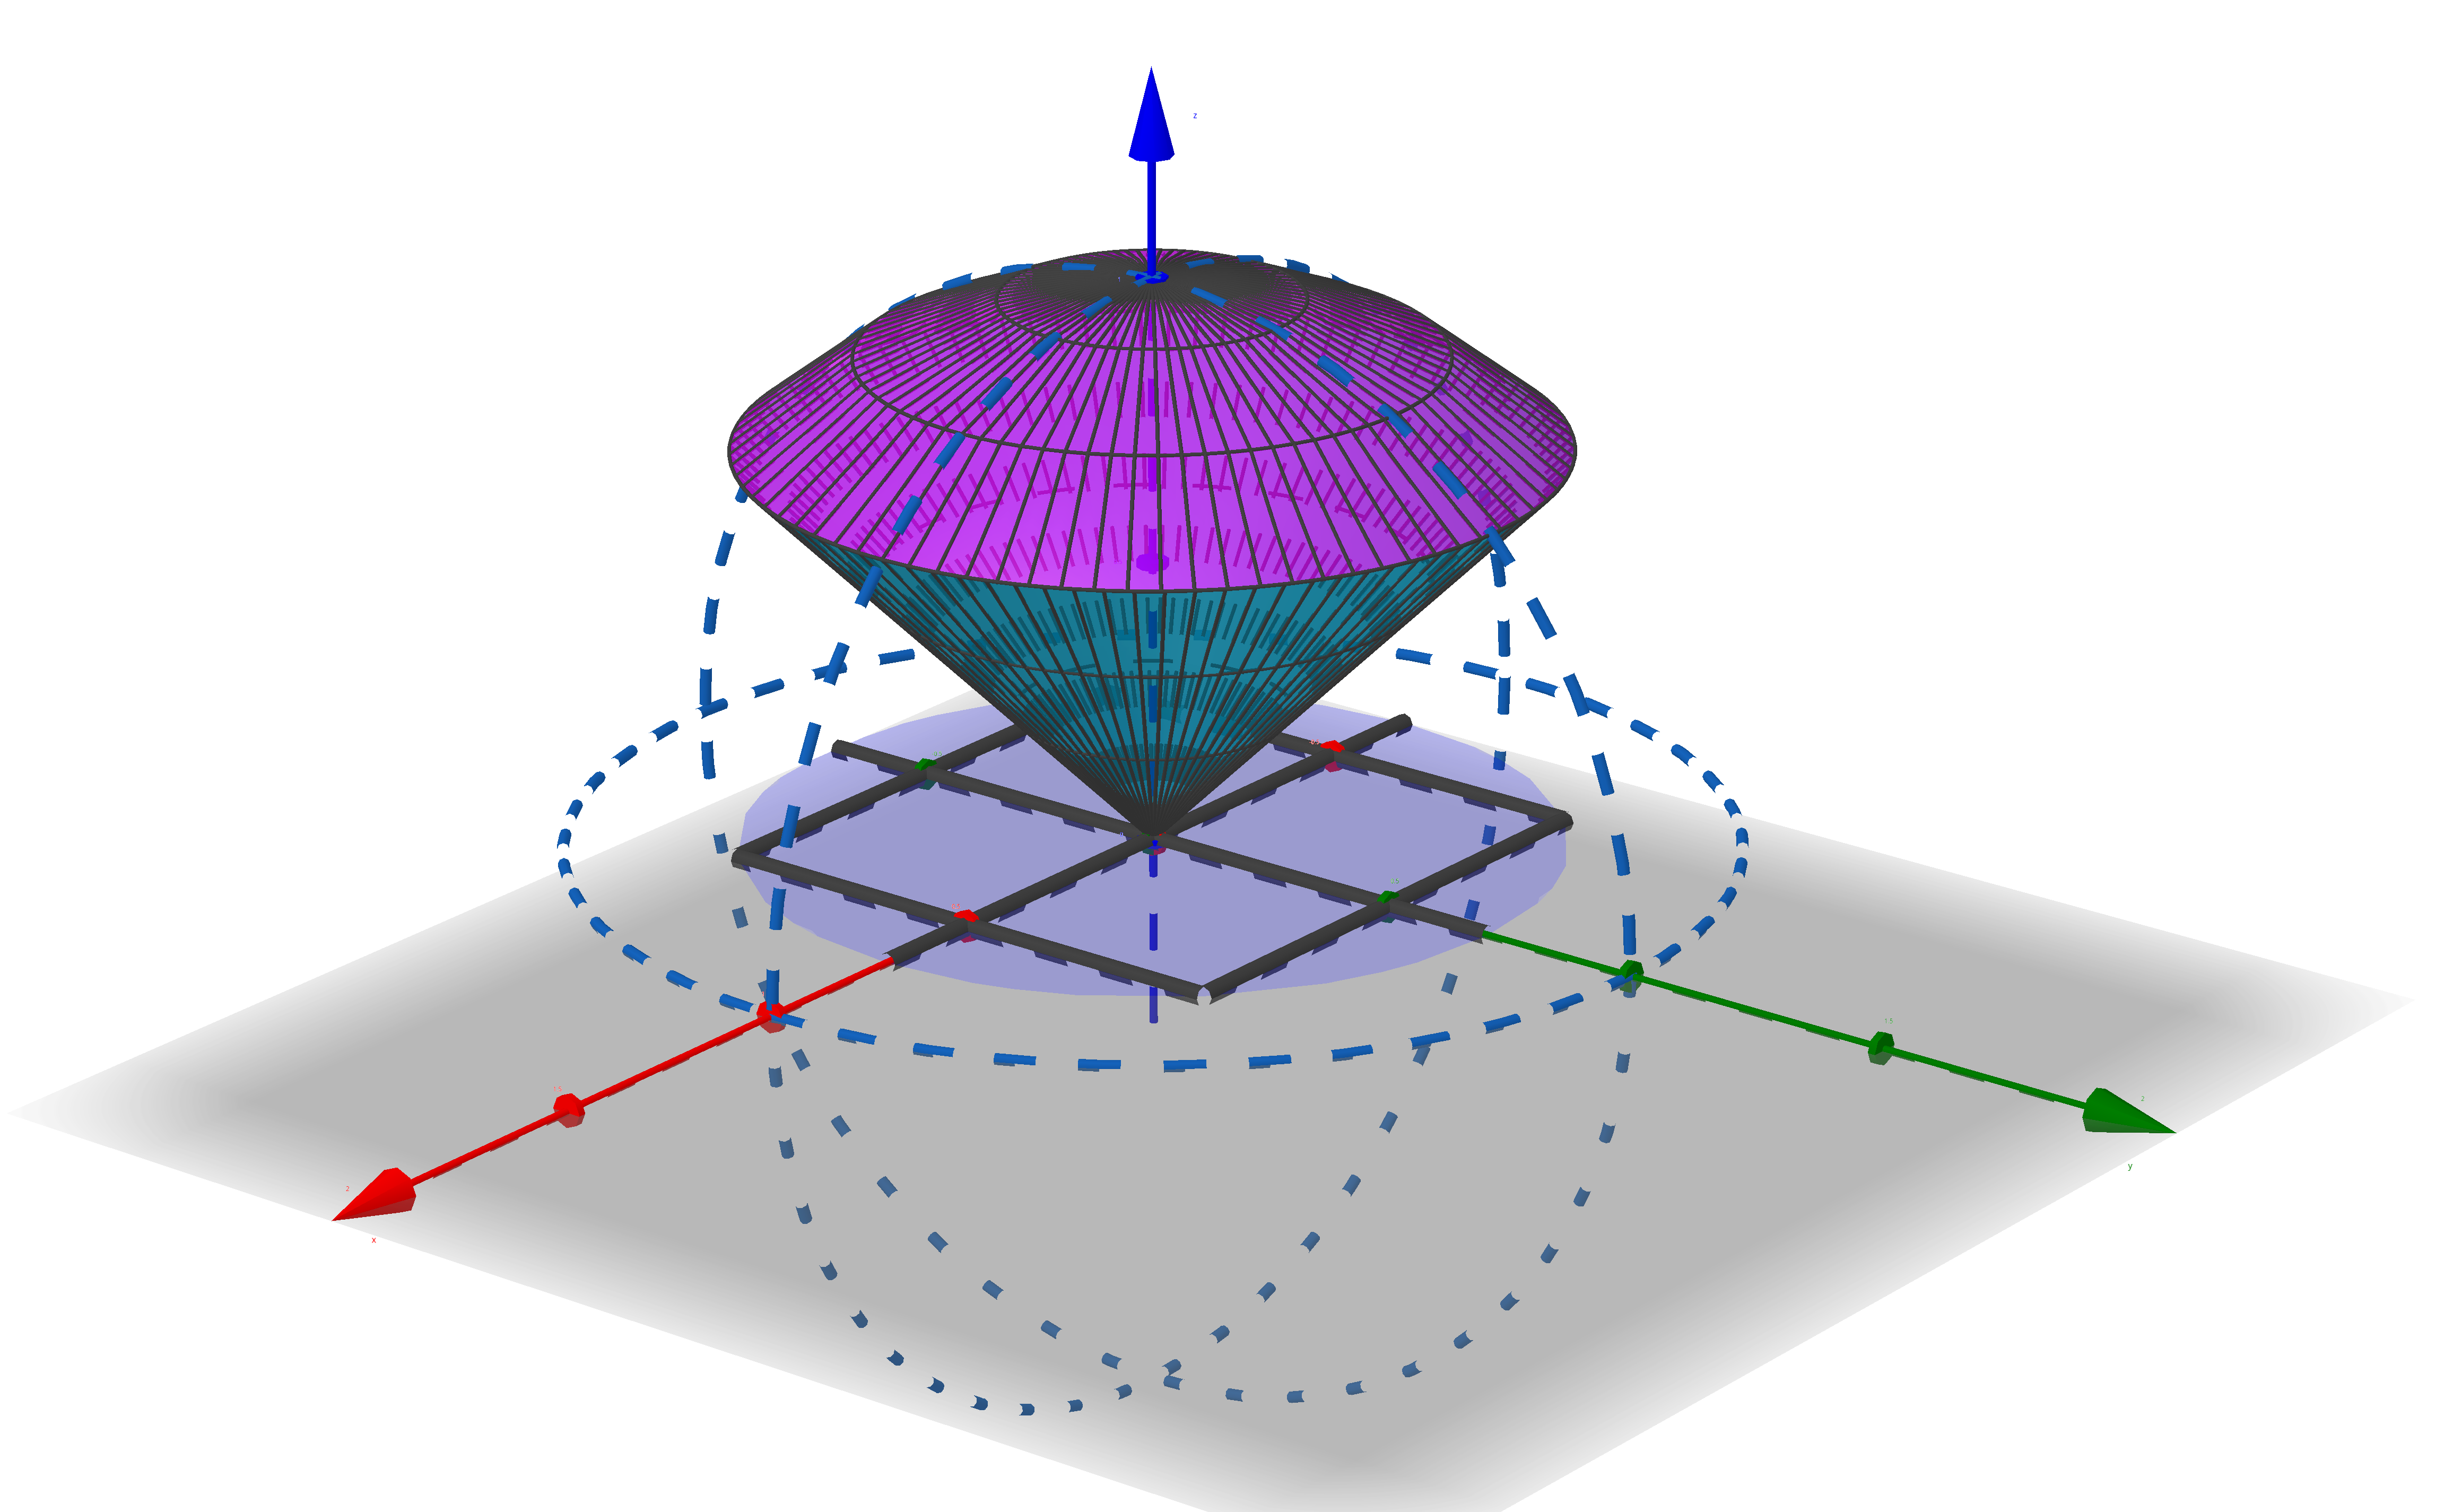
\includegraphics[width=10.0cm]{img/prova-3-nex-cone-esfera.png}
\end{center}

Considerando as relações
\[
\begin{cases}
  x = \rho \sen \phi \cos \theta\\
  y = \rho \sen \phi \sen \theta\\
  z = \rho \cos \phi\\
  x^2 + y^2 + z^2 = \rho^2
\end{cases}
\]
entre coordenadas esféricas e cartesianas, tem-se
\[
x^2 + y^2 + z^2 \leq 1
\Leftrightarrow
\rho^2 \leq 1
\Rightarrow
\rho \leq 1
\]
e
\begin{align*}
  z \geq \sqrt{x^2 + y^2}
  & \Leftrightarrow
    \rho \cos \phi
    \geq \sqrt{(\rho \sen \phi \cos \theta)^2 + (\rho \sen \phi \sen \theta)^2} \\
  & \qquad\quad\quad\ = \sqrt{\rho^2\sen^2\phi (\cos^2 \theta + \sen^2 \theta)}
    = \sqrt{\rho^2\sen^2\phi}
    = \rho\sen\phi\\
  & \Rightarrow
  \cos \phi \geq \sen\phi
  \Rightarrow
  0 \leq \phi \leq \frac{\pi}{4}.
\end{align*}

Além disso, tem-se $0 \leq \theta \leq 2\pi$. Assim, a integral em coordenadas esféricas é:
\begin{align*}
  \iiint_{S} z \diff{V}
  & = \int_0^{2\pi} \int_0^{\pi/4} \int_0^1 \rho \cos \phi \cdot \rho^2 \sen \phi\diff{\rho}\diff{\phi}\diff{\theta} \\
  & = \int_0^{2\pi} \int_0^{\pi/4} \left( \frac{\rho^4}{4} \bigg|_{\rho=0}^1 \cos \phi \sen \phi \right) \diff{\phi}\diff{\theta}
    = \frac{1}{4} \int_0^{2\pi} \int_0^{\pi/4} \cos \phi \sen \phi\diff{\phi}\diff{\theta} \\
  & = \frac{1}{4} \int_0^{2\pi} \left( \frac{1}{2} \sen^2 \phi \bigg|_{\phi=0}^{\pi/4} \right) \diff{\theta}
  = \frac{1}{4} \int_0^{2\pi} \left( \frac{1}{2} \cdot \frac{1}{2} \right) \diff{\theta}
  = \frac{1}{16} \int_0^{2\pi} \diff{\theta} \\
  &
  = \frac{1}{16} \left( \theta \bigg|_0^{2\pi} \right)
  = \frac{1}{16} \cdot 2\pi
  = \frac{\pi}{8}.
\end{align*}

\newpage

\Exercise[title={2,0}] Represente graficamente o sólido $S$ delimitado superiormente por $z = x + 1$, inferiormente por $z = - x - 1$ e lateralmente por $x^2 + y^2 = 1$, e utilize coordenadas cilíndricas para calcular o volume de $S$.

\Answer O sólido $S$ é a porção do cilindro $x^2 + y^2 = 1$ que está situada entre os planos $z = - x - 1$ e $z = x + 1$, conforme a figura a seguir:

\begin{center}
  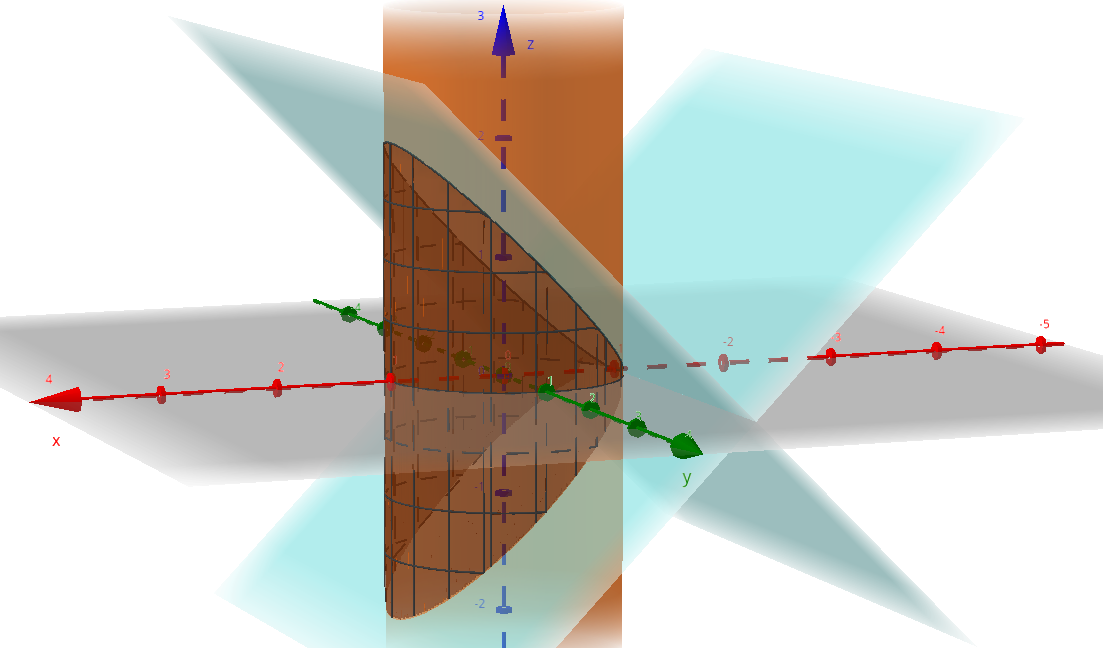
\includegraphics[width=8.0cm]{img/prova-3-nex-cilindro-e-planos.png}
\end{center}

Considerando as relações
\[
\begin{cases}
  x = r \cos \theta\\
  y = r \sen \theta\\
  z = z\\
  x^2 + y^2 = r^2
\end{cases}
\]
entre coordenadas cilíndricas e cartesianas, tem-se
\[
z = x + 1
\Leftrightarrow
z = r \cos \theta + 1,
\]
\[
z = -x - 1
\Leftrightarrow
z = -r \cos \theta - 1
\]
e
\[
x^2 + y^2 = 1
\Leftrightarrow
r^2 = 1
\Rightarrow
r = 1
\]
Ao projetar o sólido sobre o plano $xy$, obtém-se uma circunferência de raio unitário centrada na origem, o que indica que $\theta\in[0, 2\pi]$ e $r\in[0, 1]$. Então, o volume de $S$ é dado por
\begin{align*}
  \iiint_{S} 1 \diff{V}
  & = \int_0^{2\pi} \int_0^1 \int_{-r \cos \theta - 1}^{r \cos \theta + 1} 1 \cdot r \diff{z}\diff{r}\diff{\theta}
    = \int_0^{2\pi} \int_0^1 [r z] \bigg|_{z = -r \cos \theta - 1}^{z = r \cos \theta + 1} \diff{r}\diff{\theta}\\
  & = \int_0^{2\pi} \int_0^1 (r^2 \cos \theta + r)-(-r^2 \cos \theta - r) \diff{r}\diff{\theta}
    = \int_0^{2\pi} \int_0^1 2(r^2 \cos \theta + r) \diff{r}\diff{\theta}\\
  & = \int_0^{2\pi} \left(\frac{2}{3}r^3 \cos \theta + r^2\right)\bigg|_{r=0}^1 \diff{\theta}
    = \int_0^{2\pi} \frac{2}{3} \cos \theta + 1 \diff{\theta}
    = \left(\frac{2}{3} \sen \theta + \theta \right) \bigg|_{\theta=0}^{2\pi}
    = 2 \pi.
\end{align*}
\end{ExerciseList}

\begin{center}
BOA PROVA!
\end{center}

\newpage
\restoregeometry
\section*{Respostas}
\shipoutAnswer
\end{document}
